\documentclass[11pt,a4paper]{article}

\usepackage[utf8]{inputenc}
\usepackage[T1]{fontenc}
\usepackage[spanish]{babel}
\usepackage[margin=2.5cm]{geometry}
\usepackage{amsmath}
\usepackage{amssymb}
\usepackage{graphicx}
\usepackage{listings}
\usepackage{xcolor}
\usepackage{hyperref}
\usepackage{booktabs}
\usepackage{setspace}
\usepackage{parskip}

\onehalfspacing

% --- estilo para codigo Julia ---
\definecolor{juliapurple}{RGB}{100, 46, 146}
\definecolor{juliagray}{RGB}{80, 80, 80}
\definecolor{juliagreen}{RGB}{34, 139, 34}
\definecolor{juliaback}{RGB}{248, 248, 248}

\lstdefinelanguage{Julia}{
  keywords={function, return, for, in, if, end, using, import, const, do, begin, macro, struct, module},
  keywordstyle=\color{juliapurple}\bfseries,
  comment=[l]{\#},
  commentstyle=\color{juliagray}\itshape,
  stringstyle=\color{juliagreen},
  morestring=[b]",
  sensitive=true
}

\lstset{
  language=Julia,
  backgroundcolor=\color{juliaback},
  basicstyle=\ttfamily\small,
  breaklines=true,
  frame=single,
  rulecolor=\color{gray!40},
  xleftmargin=0.8em,
  xrightmargin=0.8em,
  tabsize=4
}

\hypersetup{
  colorlinks=true,
  linkcolor=blue,
  citecolor=blue,
  urlcolor=blue
}

% ============================================================
\begin{document}

\begin{center}
  {\LARGE \textbf{Regresi\'on Lineal con Gradiente Descendiente en Julia}}\\[0.3em]
  {\large Implementaci\'on Acad\'emica con Interfaz Nativa, Cuaderno Reactivo y Comparaci\'on con Biblioteca}\\[1em]
  Porfirio Sebasti\'an Rojas Ch\'avez\\
  \texttt{Porfirio.rojas0808@gmail.com}\\
  \textit{8vo Semestre --- Aprendizaje Autom\'atico}\\
  2026
\end{center}

\vspace{1em}

% ============================================================
\section*{Resumen}

Se presenta una implementaci\'on did\'actica de regresi\'on lineal univariada con gradiente descendiente en el lenguaje Julia. El trabajo se organiza en torno a dos programas principales: una aplicaci\'on de escritorio con interfaz nativa Gtk (\texttt{lineal\_regresion\_guinativa.jl}) y un cuaderno reactivo de Pluto.jl (\texttt{regresion\_pluto.jl}). Ambos construyen expl\'icitamente el modelo, la funci\'on de costo, las derivadas parciales y la regla de actualizaci\'on simult\'anea, sin recurrir a bibliotecas de aprendizaje autom\'atico. Como referencia profesional se incluye una tercera versi\'on (\texttt{regresion\_lineal\_libreria.jl}) que resuelve el mismo problema con la biblioteca \texttt{GLM.jl}, mostrando que una funci\'on de biblioteca equivale, en la pr\'actica, a fijar un conjunto de hiperpar\'ametros ya validados por otro. Para facilitar la comprensi\'on se emplea la analog\'ia de una radio antigua que debe sintonizarse girando perillas, haciendo tangibles los s\'imbolos matem\'aticos.

% ============================================================
\section{Introducci\'on}

La regresi\'on lineal es el punto de partida del aprendizaje autom\'atico: modelo parametrizado, funci\'on de costo y un algoritmo de optimizaci\'on que ajusta los par\'ametros para reducir el error \cite{ng2022ml}. Entender este caso simple es entender el esqueleto que sostiene modelos mucho m\'as grandes \cite{goodfellow2016deep}.

Este reporte documenta dos implementaciones complementarias escritas en Julia que resuelven el problema paso a paso, sin abstracciones: una con interfaz nativa Gtk y otra como cuaderno reactivo en Pluto. Una tercera implementaci\'on, basada en la biblioteca \texttt{GLM.jl}, se incluye como ejemplo de c\'omo luce el mismo problema resuelto por una biblioteca estad\'istica profesional; su inter\'es aqu\'i es pedag\'ogico, ya que permite ver que los hiperpar\'ametros que el usuario ajusta a mano en las dos primeras versiones son equivalentes a las decisiones que la biblioteca toma internamente de forma autom\'atica.

El objetivo es doble: construir un programa funcional donde el estudiante pueda modificar par\'ametros y observar el efecto en tiempo real, y hacerlo con c\'odigo lo suficientemente transparente para que cada l\'inea se corresponda con un s\'imbolo de la formulaci\'on matem\'atica.

\subsection{Analog\'ia de la radio antigua}

Antes de ir al formalismo, conviene una imagen concreta. Imag\'inese una radio muy antigua rescatada del \'atico. Se conecta y al principio solo sale ruido por la bocina; el objetivo es sintonizar una estaci\'on que s\'i se escucha con claridad. Bajo esa idea cada s\'imbolo tiene un correlato f\'isico:

\begin{itemize}
  \item $x$ (entradas): las ondas electromagn\'eticas que chocan contra la antena. Es informaci\'on del entorno que no se controla.
  \item $y$ (salida real): la canci\'on original, tal como la emite la estaci\'on. Es la meta.
  \item $f(x) = wx + b$ (predicci\'on): el sonido que efectivamente sale por la bocina en este instante.
  \item $J$ (funci\'on de costo): el dolor de cabeza de escuchar est\'atica. Mide qu\'e tan lejos est\'a el sonido real de la canci\'on deseada. El objetivo es reducirlo a cero.
  \item $m$ (n\'umero de datos): las frecuencias distintas que se prueban para asegurarse de que la radio funciona en general, no solo en un canal afortunado.
  \item $w$ (peso o pendiente): la perilla principal de sintonia. Afecta directamente c\'omo se traducen las ondas que entran en sonido.
  \item $b$ (sesgo o intercepto): el ajuste fino o la posici\'on de la antena. Sube o baja el nivel base de la se\~nal para quitar un zumbido constante.
  \item $\partial J/\partial w$, $\partial J/\partial b$ (gradientes): el o\'ido del t\'ecnico. Dicen en qu\'e direcci\'on girar cada perilla para que el ruido baje en lugar de subir.
  \item $\alpha$ (tasa de aprendizaje): la brusquedad con la que se gira la perilla. Si la mano es pesada, se pasa de la estaci\'on; si es demasiado d\'ebil, se tarda toda la noche.
  \item N\'umero de iteraciones: cu\'antos empujoncitos de paciencia se le dan a la perilla antes de parar.
\end{itemize}

El programa es, en esencia, un rob\'ot ciego que usa las derivadas como o\'idos para girar $w$ y $b$ con fuerza $\alpha$, repitiendo hasta que la canci\'on suene lo m\'as limpia posible.

% ============================================================
\section{Metodolog\'ia}

Esta secci\'on describe los fundamentos matem\'aticos del algoritmo y la estructura del c\'odigo implementado. Cada f\'ormula se acompa\~na de la funci\'on de Julia que la realiza, tomando como referencia principal la versi\'on con interfaz gr\'afica nativa (\texttt{lineal\_regresion\_guinativa.jl}).

\subsection{El modelo}

El modelo lineal univariado predice la salida como una funci\'on af\'in de la entrada:

\begin{equation}
  f_{(w,b)}(x) = wx + b
  \label{eq:modelo}
\end{equation}

donde $w$ es la pendiente y $b$ el intercepto. En la analog\'ia de la radio, $w$ es la perilla principal y $b$ el ajuste fino. En el c\'odigo esto es una l\'inea:

\begin{lstlisting}
function modelo(w, b, x)
    return w * x + b
end
\end{lstlisting}

Se escribe como funci\'on independiente para reutilizarla en la funci\'on de costo, en las derivadas y en la graficaci\'on, sin repetir la f\'ormula.

\subsection{La funci\'on de costo}

Para medir el error del modelo se usa el error cuadr\'atico medio con un factor $\tfrac{1}{2}$:

\begin{equation}
  J(w,b) = \frac{1}{2m} \sum_{i=1}^{m} \left( f_{(w,b)}\!\left(x^{(i)}\right) - y^{(i)} \right)^2
  \label{eq:costo}
\end{equation}

Elevar al cuadrado evita que errores positivos y negativos se cancelen y penaliza m\'as los errores grandes. El factor $\tfrac{1}{2}$ es conveniencia: al derivar, el $2$ del exponente se cancela con el denominador, dejando expresiones m\'as limpias. En el c\'odigo:

\begin{lstlisting}
function funcion_costo(w, b, x_datos, y_datos)
    m = length(x_datos)
    suma = sum((modelo(w, b, x_datos[i]) - y_datos[i])^2 for i in 1:m)
    return suma / (2.0 * m)
end
\end{lstlisting}

La l\'inea del \texttt{sum} es una transcripci\'on casi literal de \eqref{eq:costo}: para cada ejemplo $i$ se calcula el error, se eleva al cuadrado y se suma. Esta claridad es caracter\'istica de Julia: el bucle expl\'icito no tiene penalizaci\'on de rendimiento porque el compilador JIT lo traduce a instrucciones de m\'aquina nativas \cite{bezanson2017julia}.

\subsection{Las derivadas parciales}

Para decidir hacia d\'onde mover $w$ y $b$ se necesita la pendiente local del costo, es decir, el gradiente:

\begin{equation}
  \frac{\partial J}{\partial w} = \frac{1}{m} \sum_{i=1}^{m} \left(\hat{y}^{(i)} - y^{(i)}\right) x^{(i)}
  \label{eq:djdw}
\end{equation}

\begin{equation}
  \frac{\partial J}{\partial b} = \frac{1}{m} \sum_{i=1}^{m} \left(\hat{y}^{(i)} - y^{(i)}\right)
  \label{eq:djdb}
\end{equation}

La \'unica diferencia entre ambas es el factor $x^{(i)}$ en la de $w$, que aparece porque $\partial(wx+b)/\partial w = x$. Para $b$, como $\partial(wx+b)/\partial b = 1$, solo se promedian los errores. Las dos funciones de Julia son espejo de las f\'ormulas:

\begin{lstlisting}
function dj_dw(w, b, x_datos, y_datos)
    m = length(x_datos)
    suma = sum((modelo(w,b,x_datos[i]) - y_datos[i]) * x_datos[i] for i in 1:m)
    return suma / m
end

function dj_db(w, b, x_datos, y_datos)
    m = length(x_datos)
    suma = sum(modelo(w,b,x_datos[i]) - y_datos[i] for i in 1:m)
    return suma / m
end
\end{lstlisting}

En la analog\'ia, estas son las dos flechas que el o\'ido interno produce: una para saber c\'omo girar la perilla grande ($w$) y otra para ajustar la antena ($b$).

\subsection{Gradiente descendiente con actualizaci\'on simult\'anea}

El algoritmo se mueve en direcci\'on contraria al gradiente con paso $\alpha$:

\begin{align}
  w &\leftarrow w - \alpha \, \frac{\partial J}{\partial w} \label{eq:upw}\\
  b &\leftarrow b - \alpha \, \frac{\partial J}{\partial b} \label{eq:upb}
\end{align}

Hay un detalle importante: ambas actualizaciones deben usar los mismos valores de $w$ y $b$ en el momento de calcular las derivadas. Si se actualiza $w$ primero y luego se usa ese $w$ nuevo para calcular $\partial J/\partial b$, el resultado es incorrecto. La soluci\'on, denominada \emph{swap} en las notas, es calcular variables temporales antes de asignar:

\begin{lstlisting}
for iter in 1:num_iter
    grad_w = dj_dw(w, b, x_datos, y_datos)
    grad_b = dj_db(w, b, x_datos, y_datos)

    temp_w = w - alfa * grad_w
    temp_b = b - alfa * grad_b
    w = temp_w
    b = temp_b

    costo = funcion_costo(w, b, x_datos, y_datos)
    push!(hist_costo, costo)
    push!(hist_w, w)
    push!(hist_b, b)
end
\end{lstlisting}

En cada iteraci\'on se guardan los valores de $w$, $b$ y $J$ en tres vectores de historial. Estos historiales son esenciales para las gr\'aficas: permiten reconstruir el camino que sigui\'o el optimizador y dibujar la par\'abola de costo con la secuencia de puntos por los que pas\'o el algoritmo.

\subsection{Estabilidad num\'erica y elecci\'on de $\alpha$}

Durante el desarrollo se observ\'o que con datasets de rango grande (por ejemplo $x \in [0,100]$) el valor por defecto $\alpha = 0.01$ produc\'ia \texttt{NaN} en pocas iteraciones. La causa es directa: como $\partial J/\partial w$ incluye $x^{(i)}$, cuando los $x$ son grandes los pasos se vuelven gigantes y el algoritmo diverge. La condici\'on te\'orica de convergencia es $\alpha < 2/\mathbb{E}[x^2]$ \cite{hastie2009elements}. La tabla~\ref{tab:alpha} resume los valores seguros para los datasets considerados.

\begin{table}[h]
  \centering
  \caption{Tasa de aprendizaje m\'axima segura por dataset.}
  \label{tab:alpha}
  \begin{tabular}{@{}ccc@{}}
    \toprule
    \textbf{Dataset} & \textbf{Rango de} $x$ & \textbf{$\alpha$ m\'aximo} \\
    \midrule
    3--7 puntos manuales  & $[1,\;7]$   & $\approx 0.08$   \\
    20 puntos aleatorios  & $[0,\;20]$  & $\approx 0.015$  \\
    50 puntos aleatorios  & $[0,\;50]$  & $\approx 0.0024$ \\
    100 puntos aleatorios & $[0,\;100]$ & $\approx 0.0006$ \\
    \bottomrule
  \end{tabular}
\end{table}

Por eso la versi\'on final usa datasets peque\~nos con $x \in [1,7]$, donde $\alpha = 0.01$ e iteraciones $= 100$ convergen sin problemas. En la analog\'ia: si la mano que gira la perilla es muy brusca ($\alpha$ alto) para ondas de se\~nal grandes, la estaci\'on se pasa siempre de largo.

\subsection{Versi\'on Gtk nativa (\texttt{lineal\_regresion\_guinativa.jl})}

La primera implementaci\'on construye una ventana nativa con la biblioteca \texttt{Gtk.jl}. El archivo est\'a organizado de abajo hacia arriba en orden de abstracci\'on creciente: primero los datos constantes, luego \texttt{modelo}, \texttt{funcion\_costo}, \texttt{dj\_dw}, \texttt{dj\_db}, despu\'es \texttt{gradiente\_descendiente}, luego \texttt{graficar}, y finalmente \texttt{lanzar\_aplicacion} que es la GUI. Cada funci\'on solo usa funciones definidas antes.

La interfaz tiene cuatro campos de par\'ametros (\texttt{alfa}, iteraciones, paso de muestreo de rectas, m\'aximo de rectas en la gr\'afica de evoluci\'on), cuatro botones con datasets predefinidos de 3, 5, 6 y 7 puntos, una secci\'on de entrada manual (dos campos de texto con valores separados por coma) y un panel de resultados. Al presionar cualquier bot\'on se ejecuta el ciclo: leer par\'ametros, llamar a \texttt{gradiente\_descendiente}, calcular el costo final, mostrarlo en el panel y llamar a \texttt{graficar}.

Las gr\'aficas se muestran en el navegador usando el backend \texttt{plotlyjs()}, que permite zoom, desplazamiento y tooltips con los valores exactos bajo el cursor. La figura final tiene cuatro paneles en cuadr\'icula $2\times 2$:

\begin{enumerate}
  \item \textbf{Regresi\'on ajustada:} los puntos originales y la recta final $f^{*}(x) = w^{*}x + b^{*}$.
  \item \textbf{Evoluci\'on de las rectas:} un abanico de rectas intermedias tomadas cada \texttt{paso\_recta} iteraciones, en tonos de azul que pasan de claro (primeras) a oscuro (\'ultimas), con la recta \'optima superpuesta en rojo discontinuo.
  \item \textbf{Par\'abola de costo:} $J(w, b^{*})$ como funci\'on de $w$, con los puntos naranja que marcan la posici\'on de $w$ en cada iteraci\'on del algoritmo y un diamante verde en el m\'inimo. Esta es la superficie de costo.
  \item \textbf{Convergencia:} $J(w,b)$ contra el n\'umero de iteraci\'on, con la t\'ipica curva de decaimiento exponencial que baja r\'apido al inicio y se aplana.
\end{enumerate}

Es importante no confundir los paneles 3 y 4. El panel 4 muestra c\'omo el costo cambia \emph{en el tiempo} (el proceso); el panel 3 muestra la \emph{forma geom\'etrica} de la funci\'on de costo (el espacio). El panel 3 es la raz\'on visual por la que el algoritmo funciona: la superficie tiene forma de taz\'on convexo, sin m\'inimos locales, y bajar siempre en direcci\'on del gradiente necesariamente lleva al fondo.

\subsection{Versi\'on Pluto reactiva (\texttt{regresion\_pluto.jl})}

La segunda implementaci\'on es un cuaderno de \texttt{Pluto.jl} \cite{plutojl} que reimplementa las mismas funciones matem\'aticas, pero reemplaza toda la GUI por widgets \texttt{@bind}:

\begin{lstlisting}
md"""**learning rate (alfa):** $(@bind alfa
     NumberField(0.0001:0.0001:1.0, default=0.01))"""
md"""**numero de iteraciones:** $(@bind iters
     NumberField(10:10:10000, default=100))"""
md"""**conjunto de datos:** $(@bind ds
     Select(["3 puntos","5 puntos","6 puntos",
             "7 puntos","manual"], default="5 puntos"))"""
\end{lstlisting}

A diferencia de Jupyter, Pluto es estrictamente reactivo: cambiar cualquier control dispara autom\'aticamente la re-ejecuci\'on de todas las celdas que dependen de ese valor, sin necesidad de presionar ning\'un bot\'on. As\'i, mover el \texttt{NumberField} de $\alpha$ re-entrena el modelo y redibuja las cuatro gr\'aficas al instante, lo que permite observar de primera mano c\'omo una tasa de aprendizaje muy alta hace que el optimizador rebote sobre la par\'abola, o c\'omo una muy baja lo deja a medio camino despu\'es de 100 iteraciones.

La l\'ogica matem\'atica es id\'entica a la de la versi\'on Gtk: mismas funciones \texttt{modelo}, \texttt{funcion\_costo}, \texttt{dj\_dw}, \texttt{dj\_db} y \texttt{gradiente\_descendiente}. Lo que cambia es el envoltorio: unas 150 l\'ineas de c\'odigo GUI en Gtk se convierten en cero l\'ineas de GUI en Pluto, reemplazadas por seis directivas \texttt{@bind}. El cuaderno tambi\'en usa \texttt{import PlotlyJS} (en lugar de \texttt{using}) para evitar un conflicto de nombres con \texttt{Plots.scatter}.

\subsection{Versi\'on con biblioteca (\texttt{regresion\_lineal\_libreria.jl})}

La tercera implementaci\'on es solo de contraste. Resuelve el problema en una sola llamada a \texttt{GLM.jl}:

\begin{lstlisting}
using GLM, DataFrames
function ajustar_modelo(x_datos, y_datos)
    df = DataFrame(X = x_datos, Y = y_datos)
    return lm(@formula(Y ~ X), df)
end
\end{lstlisting}

Internamente resuelve las ecuaciones normales $\boldsymbol{\theta}^{*} = (\mathbf{X}^{\top}\mathbf{X})^{-1}\mathbf{X}^{\top}\mathbf{y}$ mediante factorizaci\'on QR, obteniendo la soluci\'on \'optima exacta en una sola operaci\'on matricial. No requiere $\alpha$ ni n\'umero de iteraciones porque no es iterativa.

Esta versi\'on no pretende ense\~nar el algoritmo, sino mostrar c\'omo se trabaja con bibliotecas: el usuario ya no decide los hiperpar\'ametros, estos est\'an resueltos internamente por quienes implementaron \texttt{GLM.jl}. En ese sentido, \emph{usar una biblioteca es casi equivalente a aceptar un conjunto de hiperpar\'ametros ya validados}: el estudiante no toca $\alpha$ ni las iteraciones porque alguien m\'as ya hizo el trabajo de elegir una estrategia num\'ericamente estable. De ah\'i el valor de haber implementado primero la versi\'on manual: quien entiende el c\'odigo de \texttt{lineal\_regresion\_guinativa.jl} puede leer despu\'es la documentaci\'on de \texttt{GLM.jl} sabiendo exactamente qu\'e abstrae la biblioteca.

% ============================================================
\section{Resultados}

Los tres programas producen resultados consistentes entre s\'i. Con los datasets manuales en $x \in [1,7]$ y $\alpha = 0.01$, $100$ iteraciones, el gradiente descendiente converge a pendientes cercanas a $1.3$--$1.5$ e interceptos cercanos a $0.3$--$0.7$, seg\'un el dataset. La versi\'on con GLM sobre los mismos puntos devuelve valores ligeramente distintos pero dentro del mismo orden, confirmando que ambos m\'etodos encuentran esencialmente la misma recta.

En la versi\'on Gtk, el panel de par\'abola de costo muestra con claridad c\'omo los puntos naranjas, inicialmente espaciados en la parte alta de la curva, se acumulan en el vado cerca del m\'inimo a medida que avanzan las iteraciones. En la versi\'on Pluto, mover el campo de $\alpha$ entre $0.005$ y $0.08$ (el m\'aximo seguro aproximado para este rango de datos) basta para reproducir el fen\'omeno completo, desde una convergencia lenta hasta oscilaciones previas al colapso num\'erico.

El abanico de rectas del panel 2 muestra que las primeras iteraciones producen rectas casi horizontales cerca del origen (porque $w$ y $b$ arrancan en cero) y que la pendiente y el intercepto se aproximan progresivamente a sus valores \'optimos, acumul\'andose al final cerca de la recta roja discontinua que marca la soluci\'on.

\subsection{Cuatro experimentos ilustrativos}

Para hacer concretos los conceptos anteriores, se ejecutaron cuatro corridas del programa \texttt{regresion\_pluto.jl} con configuraciones elegidas para exponer comportamientos opuestos: dos casos de convergencia exitosa y dos de fallo del optimizador. En cada figura, la captura superior muestra los par\'ametros ingresados; las dos im\'agenes inferiores muestran, a la izquierda, la recta ajustada y la superficie de costo $J(w)$, y a la derecha, la evoluci\'on de las rectas intermedias y la curva de convergencia.

\subsubsection*{Caso 1 --- Convergencia r\'apida (3~puntos, $\alpha = 0.01$, 300~iteraciones)}

\begin{figure}[h!]
  \centering
  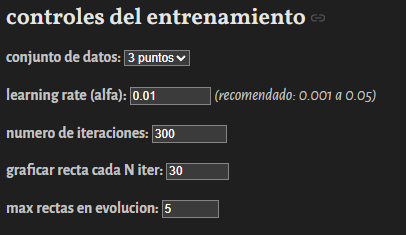
\includegraphics[width=0.60\linewidth]{3_01_300_30_5.png}\\[0.6em]
  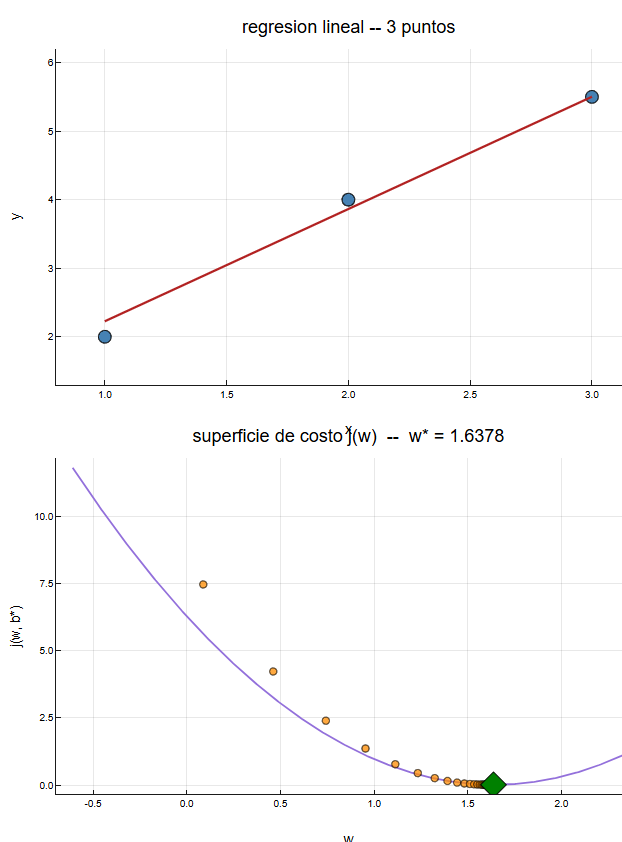
\includegraphics[width=0.47\linewidth]{3_01_300_30_5(2).png}
  \hspace{0.04\linewidth}
  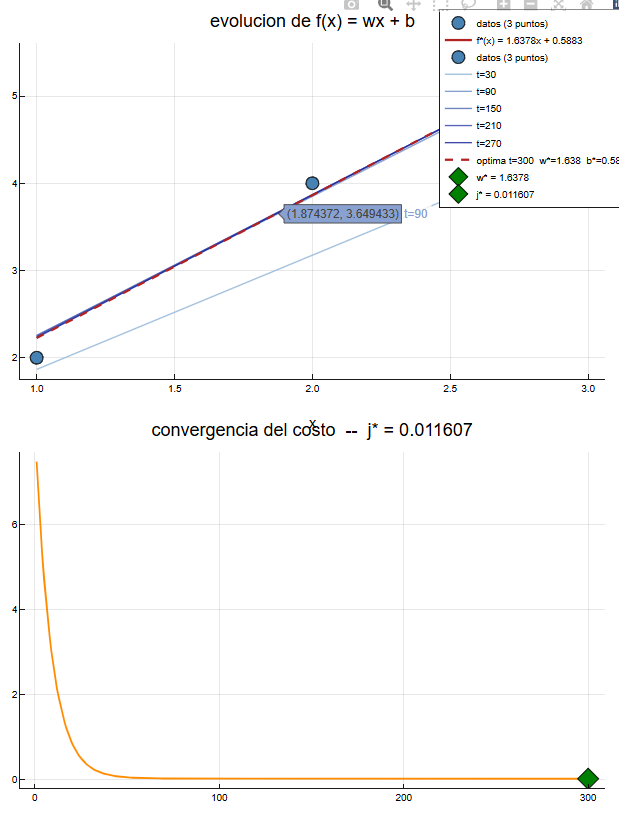
\includegraphics[width=0.47\linewidth]{3_01_300_30_5(3).png}
  \caption{Caso~1: convergencia exitosa con 3~puntos, $\alpha = 0.01$ y 300~iteraciones. La recta ajustada pasa cerca de los tres puntos. En la par\'abola los puntos naranjas se acumulan en el m\'inimo (diamante verde, $w^{*} \approx 1.64$). La curva de convergencia baja r\'apido y se aplana, indicando que el algoritmo lleg\'o al fondo con costo final $J^{*} \approx 0.012$.}
  \label{fig:caso1}
\end{figure}

Con un dataset peque\~no y una tasa moderada el algoritmo no tiene dificultad. La curva de costo desciende de forma casi exponencial en las primeras cincuenta iteraciones y luego se aplana. En la analog\'ia de la radio, es girar la perilla con pulso firme: pocos movimientos y casi todo el ruido desaparece. Los puntos naranjas en la par\'abola ilustran el recorrido de $w$ desde el origen hasta el m\'inimo, donde la derivada se anula y el algoritmo deja de moverse.

\subsubsection*{Caso 2 --- Convergencia gradual (7~puntos, $\alpha = 0.003$, 300~iteraciones)}

\begin{figure}[h!]
  \centering
  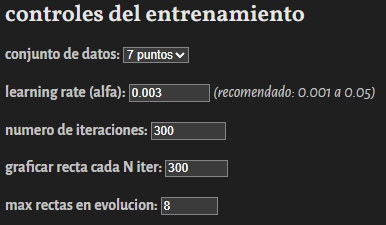
\includegraphics[width=0.60\linewidth]{7_003_300_300_8.png}\\[0.6em]
  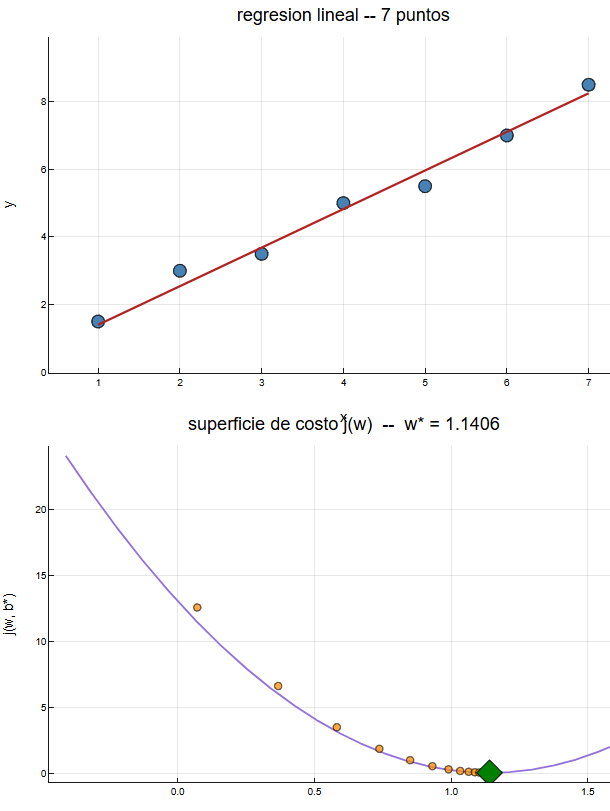
\includegraphics[width=0.47\linewidth]{7_003_300_300_8(2).png}
  \hspace{0.04\linewidth}
  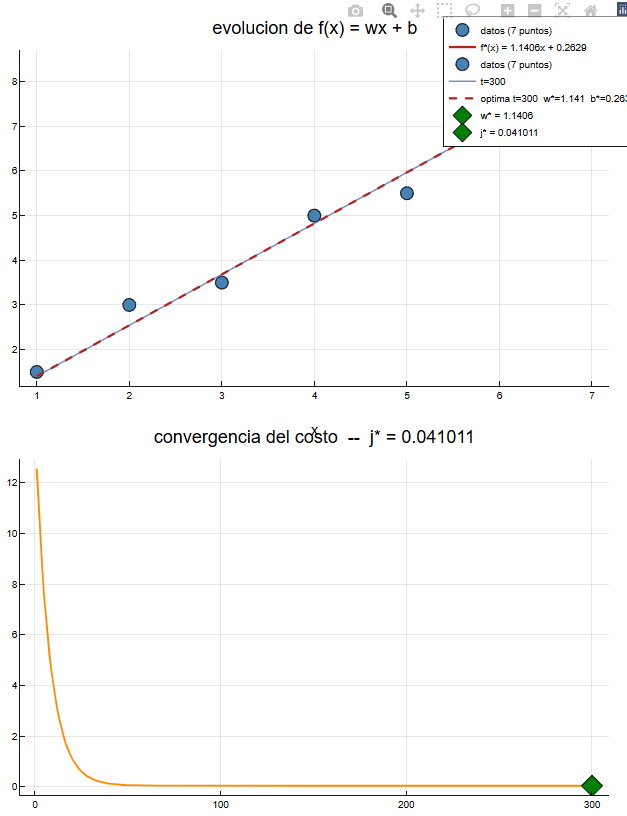
\includegraphics[width=0.47\linewidth]{7_003_300_300_8(3).png}
  \caption{Caso~2: convergencia exitosa con 7~puntos, $\alpha = 0.003$ y 300~iteraciones. La recta cubre bien los siete puntos y el m\'inimo queda en $w^{*} \approx 1.14$. Los pasos son m\'as peque\~nos que en el caso~1 porque $\alpha$ es menor, pero el destino es el mismo: el fondo de la par\'abola.}
  \label{fig:caso2}
\end{figure}

Al ampliar el dataset a 7~puntos, el gradiente $\partial J/\partial w$ acumula t\'erminos multiplicados por valores de $x$ hasta~7, lo que agranda los pasos impl\'icitamente. Reducir $\alpha$ de $0.01$ a $0.003$ compensa ese efecto \cite{hastie2009elements}. La convergencia es igualmente correcta pero m\'as lenta; la recta final se ajusta bien a los siete puntos y la par\'abola muestra el mismo patr\'on de descenso escalonado hasta el m\'inimo.

\subsubsection*{Caso 3 --- Divergencia por $\alpha$ excesivo (7~puntos, $\alpha = 0.2$, 50~iteraciones)}

\begin{figure}[h!]
  \centering
  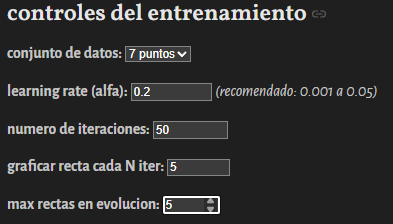
\includegraphics[width=0.60\linewidth]{7_2_50_5_5.png}\\[0.6em]
  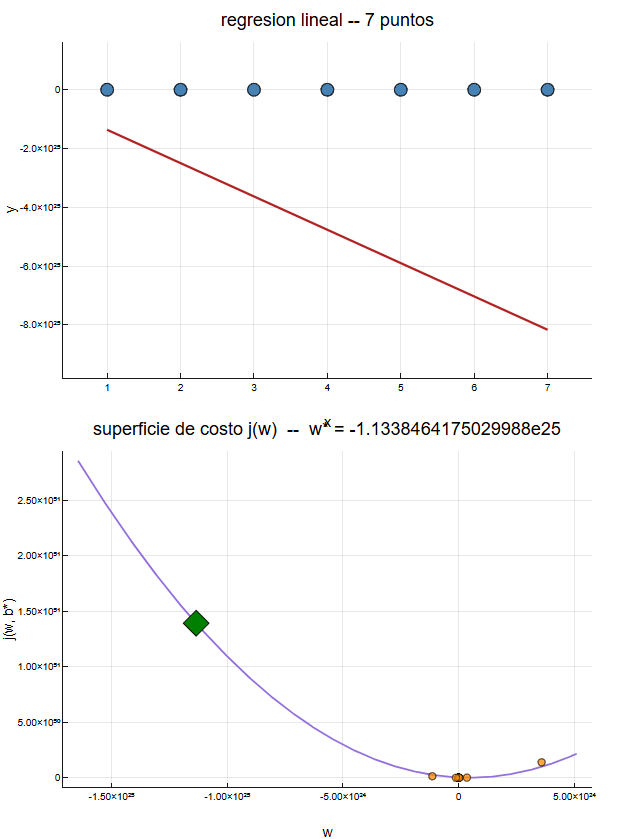
\includegraphics[width=0.47\linewidth]{7_2_50_5_5(2).png}
  \hspace{0.04\linewidth}
  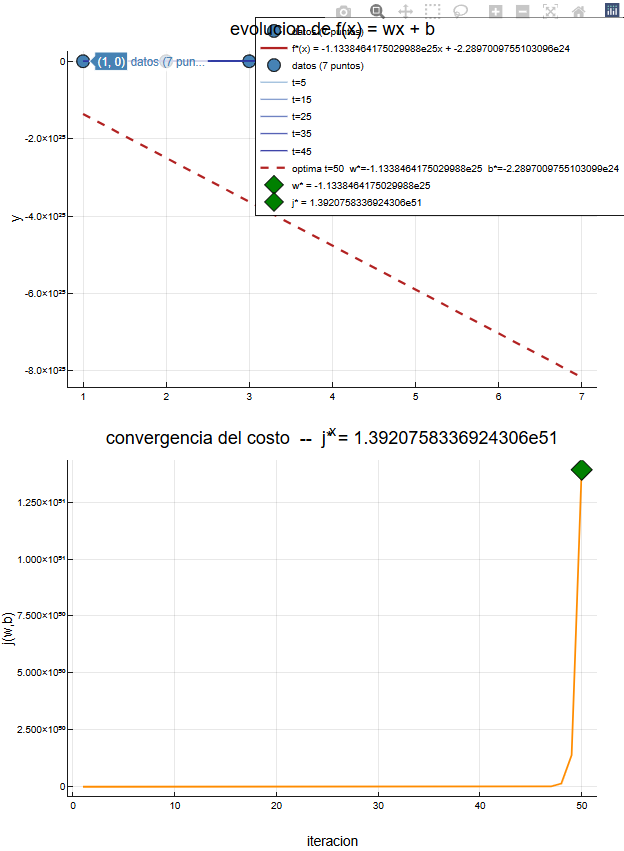
\includegraphics[width=0.47\linewidth]{7_2_50_5_5(3).png}
  \caption{Caso~3: divergencia con 7~puntos, $\alpha = 0.2$ y 50~iteraciones. Los datos originales quedan invisibles porque el eje $y$ escala hasta $10^{25}$. La curva de convergencia permanece casi plana durante~40 iteraciones y luego explota hasta $J^{*} \approx 1.39 \times 10^{51}$; los valores finales son $w^{*} \approx -1.13 \times 10^{25}$, sin significado f\'isico.}
  \label{fig:caso3}
\end{figure}

Este es el caso de la mano demasiado brusca. Con $\alpha = 0.2$ cada actualizaci\'on de $w$ produce un salto que sobrepasa el m\'inimo; el siguiente salto es a\'un mayor en la direcci\'on contraria, y la secuencia diverge. Las gr\'aficas lo confirman: los ejes escalan hasta $10^{25}$, los datos originales quedan aplastados en $y \approx 0$ a esa escala, y la curva de costo explota en las \'ultimas iteraciones en lugar de bajar. En la analog\'ia, la mano es tan brusca que la perilla pasa la estaci\'on, rebota al otro lado, cada vez m\'as lejos.

\subsubsection*{Caso 4 --- Iteraciones insuficientes (5~puntos, $\alpha = 0.005$, 8~iteraciones)}

\begin{figure}[h!]
  \centering
  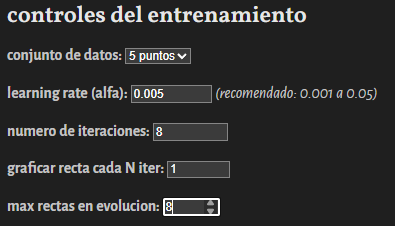
\includegraphics[width=0.60\linewidth]{5_005_8_1_8.png}\\[0.6em]
  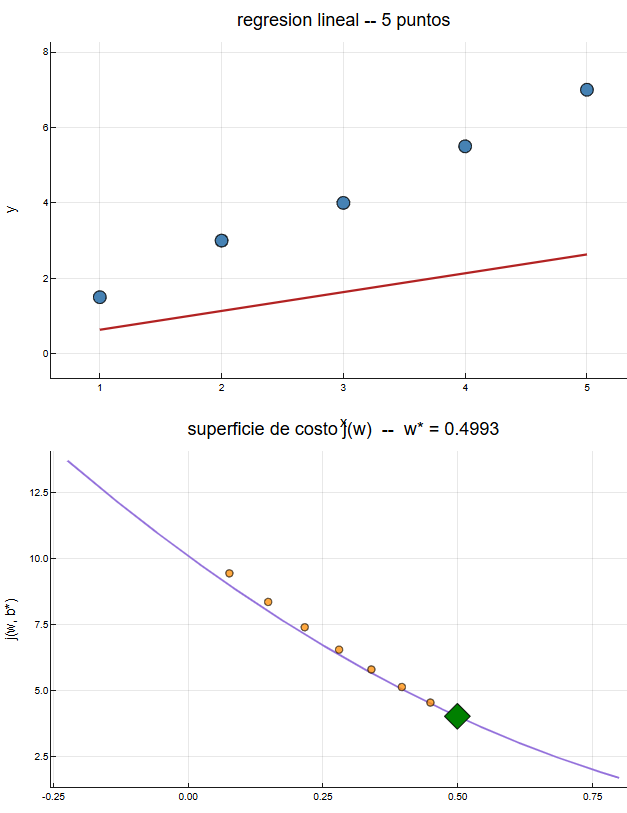
\includegraphics[width=0.47\linewidth]{5_005_8_1_8(2).png}
  \hspace{0.04\linewidth}
  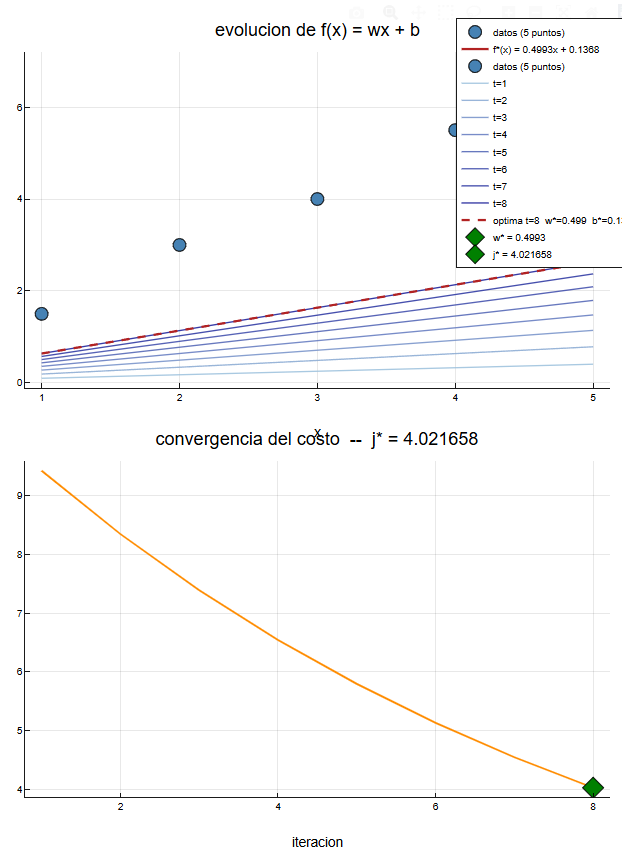
\includegraphics[width=0.47\linewidth]{5_005_8_1_8(3).png}
  \caption{Caso~4: convergencia incompleta con 5~puntos, $\alpha = 0.005$ y 8~iteraciones. La recta queda casi horizontal y por debajo de todos los datos ($w^{*} \approx 0.50$ en lugar del \'optimo $\approx 1.4$). El diamante verde aparece a mitad de la ladera de la par\'abola y la curva de costo sigue descendiendo en la \'ultima iteraci\'on: el algoritmo se detuvo antes de llegar.}
  \label{fig:caso4}
\end{figure}

Aqu\'i el problema no es la tasa de aprendizaje sino la paciencia. Con solo 8~iteraciones el algoritmo apenas comienza a bajar por la par\'abola: el diamante verde queda a mitad de la ladera ($w \approx 0.50$), la recta resultante es casi horizontal y falla en acercarse a los datos. La curva de convergencia es la se\~nal definitiva: sigue cayendo en la \'ultima iteraci\'on sin ning\'un indicio de haberse aplanado. En la analog\'ia, es darle ocho clics a la perilla, notar que la est\'atica baja, y apagar el aparato antes de llegar a la estaci\'on.

% ============================================================
\section{An\'alisis y Discusi\'on}

El ejercicio hace visible algo que las explicaciones puramente matem\'aticas suelen dejar en el abstracto: el gradiente descendiente es, literalmente, un procedimiento para rodar hacia abajo por una superficie convexa. El panel 3 de la gr\'afica es una prueba visual de ese hecho. La par\'abola existe, tiene un \'unico m\'inimo, y los puntos naranja bajan por ella; no hay misterio ni magia.

La eleccci\'on de Julia como lenguaje no es incidental. El compilador JIT especializado por tipos permite escribir bucles como \texttt{sum((modelo(w,b,x[i]) - y[i])*x[i] for i in 1:m)}, transcripci\'on casi textual de la f\'ormula, sin la penalizaci\'on de rendimiento que este c\'odigo tendr\'ia en Python puro \cite{bezanson2017julia}. En Python habr\'ia que vectorizar con NumPy y reescribir el algoritmo en t\'erminos matriciales, alej\'andolo de la f\'ormula original. En Julia el estudiante puede leer el c\'odigo como lee la derivada.

La comparaci\'on entre las tres versiones ilumina la econom\'ia de las bibliotecas. La versi\'on manual en Gtk tiene alrededor de 500 l\'ineas; la versi\'on Pluto reduce la GUI a casi nada y queda en torno a 300 l\'ineas; la versi\'on con GLM cabe en menos de 100 l\'ineas porque el trabajo lo hace \texttt{lm}. Pero la reducci\'on de l\'ineas oculta decisiones: qu\'e algoritmo num\'erico usar, c\'omo evitar divergencia, qu\'e tolerancia aceptar. Esas decisiones son los hiperpar\'ametros que el usuario de la biblioteca no ve. En la versi\'on manual, se ven todos.

El costo es que la versi\'on manual puede explotar: con datasets de rango amplio y $\alpha$ mal elegido, aparecen \texttt{NaN}. La biblioteca no tiene ese problema. Ambas cosas son ciertas y el contraste es el aprendizaje.

Desde la perspectiva del aprendizaje autom\'atico m\'as amplio, el valor del gradiente descendiente no est\'a en este caso particular ---donde OLS es m\'as r\'apido y m\'as estable--- sino en que es el mismo m\'etodo que entrena redes neuronales, modelos log\'isticos y transformadores. Lo que cambia es el tama\~no del modelo y la funci\'on de costo, no la l\'ogica iterativa \cite{goodfellow2016deep}. Implementarlo a mano en el caso m\'as simple es una inversi\'on con rendimiento desproporcionado: se entiende el esqueleto sobre el que se apoya el resto de la disciplina.

% ============================================================
\section{Conclusiones}

El trabajo entrega dos implementaciones funcionales y una referencia. \texttt{lineal\_regresion\_guinativa.jl} ofrece una experiencia de escritorio con entrenamiento bajo demanda y gr\'aficas interactivas en el navegador; \texttt{regresion\_pluto.jl} replica la misma matem\'atica en un cuaderno reactivo donde cualquier cambio de par\'ametro recalcula todo autom\'aticamente; \texttt{regresion\_lineal\_libreria.jl} resuelve el problema con \texttt{GLM.jl} y sirve para ver que usar bibliotecas es, en la pr\'actica, adoptar un conjunto de decisiones ya tomadas.

La analog\'ia de la radio sostiene todo el recorrido: $w$ es la perilla, $b$ la antena, $J$ el dolor de cabeza por la est\'atica, $\alpha$ la brusquedad de la mano, y el gradiente el o\'ido que indica hacia d\'onde girar. Al final, el estudiante deber\'ia poder leer las cuatro gr\'aficas, asociar cada una con un paso del algoritmo, y entender por qu\'e esa misma estructura aparece despu\'es en modelos mucho m\'as grandes. Esa traducci\'on directa entre f\'ormula, c\'odigo e imagen es el aporte principal del ejercicio.

% ============================================================
\begin{thebibliography}{6}

\bibitem{ng2022ml}
A.~Ng, \textit{Machine Learning Specialization}. Coursera / DeepLearning.AI, 2022. [En l\'inea]. Disponible en: \url{https://www.coursera.org/specializations/machine-learning-introduction}

\bibitem{bezanson2017julia}
J.~Bezanson, A.~Edelman, S.~Karpinski, y V.~B.~Shah, ``Julia: A fresh approach to numerical computing,'' \textit{SIAM Review}, vol.~59, no.~1, pp.~65--98, 2017.

\bibitem{hastie2009elements}
T.~Hastie, R.~Tibshirani, y J.~Friedman, \textit{The Elements of Statistical Learning}, 2nd~ed. New York, NY, USA: Springer, 2009.

\bibitem{goodfellow2016deep}
I.~Goodfellow, Y.~Bengio, y A.~Courville, \textit{Deep Learning}. Cambridge, MA, USA: MIT Press, 2016.

\bibitem{plutojl}
F.~van~der~Plas \textit{et al.}, \textit{Pluto.jl: simple reactive notebooks for Julia}, 2024. [En l\'inea]. Disponible en: \url{https://plutojl.org}

\bibitem{glmjl}
D.~Bates \textit{et al.}, \textit{GLM.jl: Generalized linear models in Julia}, Julia Statistics, 2024. [En l\'inea]. Disponible en: \url{https://github.com/JuliaStats/GLM.jl}

\end{thebibliography}

\end{document}
